\section{In-video Quiz ON/OFF}

\subsection*{Problem Summary}

\hspace{0.35cm} Videos on Bodhitree are the primary learning elements. Several videos have in-video quizzes in them which pop up while the video is playing and interrupt the play. The user then has to attempt the quiz and then he can resume the video.
\par It may happen that the user has already attempted the quizzes and is watching the video again. In such instances it is desirable for the user to have an uninterrupted playback of the video(without the in-video quizzes).
\par There must be a feature which enables the user to turn the in-video quizzes on or off, thus providing a seamless playback of the video.

\subsection*{Specifications}

\begin{enumerate}
	\item A button must be present which is easily accessible on the video page and which provides the functionality to turn the video markers on or off with a single click.
	\item The button should not affect the navigation options that are present for the video in the table of contents. The user must still be able to use the markers to seek through the video.
\end{enumerate}

\subsection*{System Design}

\subsubsection*{In-video quizzes toggle Button UI}
\begin{enumerate}
	\item A button was created using CSS and Javascript to turn the video markers ON or OFF. It was placed directly under the video such that it is easily accessible as shown below in figure \ref{fig:video-popup}.

	\begin{figure}[h]
	\centering
	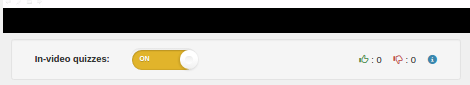
\includegraphics[width=0.95\linewidth]{./media/video_popup}
	\caption{Button to toggle the in-video quizzes ON/OFF}
	\label{fig:video-popup}
	\end{figure}

\end{enumerate}

\subsubsection*{Mechanism to toggle the video markers}
\begin{enumerate}
	\item The video container is a component created in React.js  which controls the display and playback of the video.
	\item The video markers (containing the in-video quizzes as well as the navigation options) are passed as properties to the video container.
	\item When the video container loads, a check is performed whether the \textit{in-video quizzes} toggle button is set to ON or OFF.
	\item In case the button is OFF, then markers are not passed to the video container and hence the video is played without any in-video quizzes popping up.
	\item When the button is switched back to ON, then the video container will reload the video properties along with the markers and the video will now have the in-video quizzes.
\end{enumerate}

\newpage

\section{Setting importance to threads}

\subsection*{Problem Summary}

\hspace{0.35cm} The threads in discussion forum are sorted such that the recent threads will be displayed first. There are several options to sort the threads based on their `popularity' and `earlier first'.
\par In some cases a thread has a higher importance than the others. Such a thread must be displayed at the top and there must be an option to sort the threads based on their value of importance.

\subsection*{Specification}

\begin{enumerate}
	\item Whenever a new thread is added, the default importance value should be 0.
	\item The instructor must be able to set the importance value which can be any number between 0 and 10.
	\item Any user who can view the discussion forum must be able to sort the threads according to their importance value.
\end{enumerate}

\subsection*{System Design}

\begin{enumerate}
	\item When a user is logged in with instructor privileges, a link to set the importance value is available for each thread.
	\item Once a value is set, it appears on the thread under a star symbol which denotes the importance value of that thread.
	\item If the value is not between the specified range then an error message is shown, while the importance value remains as it was earlier.
	\item A button to sort the threads based on the importance value is available to all the users.
	\item The complete UI for setting the importance, sorting the threads based on the importance value and displaying the importance value of each thread is shown in figure \ref{fig:set-importance}.
	
	\newpage
	
	\begin{figure}[h]
		\centering
		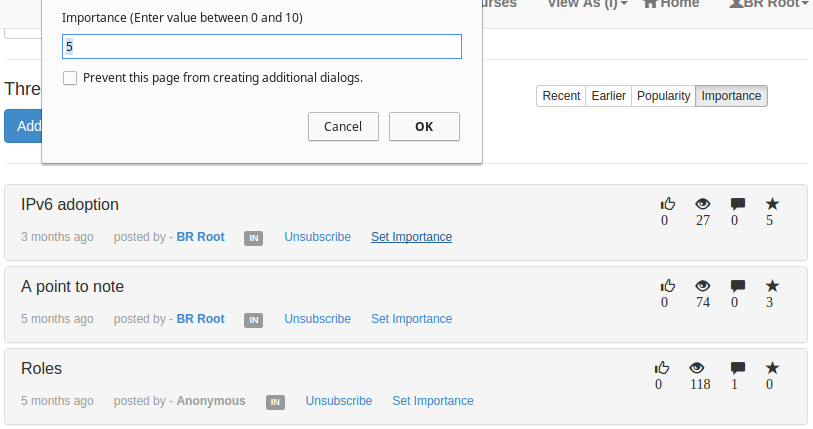
\includegraphics[width=0.95\linewidth]{./media/set_importance}
		\caption{Setting the importance value to threads}
		\label{fig:set-importance}
	\end{figure}
		
\end{enumerate}

\newpage

\section{Mail to instructor on addition of a new thread}

\subsection*{Problem Summary}

\hspace{0.35cm} Bodhitree offers discussion forums where the users can start a thread and post their queries while the other users can comment on those threads. Some of the threads are started by the instructors to post important notifications whereas many other threads are started by the students seeking help in certain aspects of the course.
\par Sometimes the threads started by the students require immediate attention of the instructor, but the instructor of that course can be aware of the thread only when he logs into Bodhitree and checks the discussion forums.
\par It is important that the instructor must be notified about the thread so that he is aware of the discussions that are happening on Bodhitree related to his course.

\subsection*{Specifications}

\hspace{0.35cm} Whenever a user starts a thread in the discussion forum, an email must be sent to the instructor and the TAs of the course.

\subsection*{System Design}

\begin{enumerate}
	\item Whenever a new thread has been added to the discussion forum of a course, a function is called which fetches all the instructors of the course (course creator as well as the TAs).
	\item The function \textbf{ArchivableEmailMessage()} then sends an email to all the fetched instructors of the course with the subject of the email as \textit{``Course title: Thread title''} and the body of the email as a hyperlink to the thread.
	\item A sample email received by the instructor is shown in figure \ref{fig:instructor-email}
	\begin{figure}[h]
	\centering
	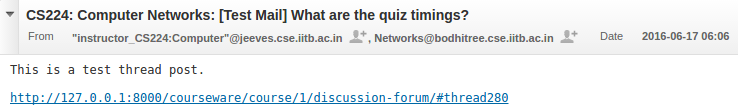
\includegraphics[width=0.95\linewidth]{./media/instructors_mail}
	\caption{Email notification to the instructors on addition of a new thread}
	\label{fig:instructor-email}
	\end{figure}
	
\end{enumerate}